% !TEX root = ../paper.tex

\section{Results}

\subsection{Pairwise Infrared-Visible Homography Evidence}

Pairwise infrared-visible homography evidence is broadly available on UAV-TAlign-12K.
Table~\ref{tab:pairwise_baselines} reports the full 6,037-pair official evaluation split.
Classical keypoint baselines provide useful but less complete pairwise evidence: SIFT and AKAZE
reach 87.08\% and 94.29\% homography availability, respectively. This provides a classical
keypoint reference, while modern dense and learned matchers further improve pairwise availability
under infrared-visible appearance gaps. Raw MINIMA and RoMa produce homographies for all pairs,
while the accepted LoFTR retry and XoFTR remain near-saturated under the same manifest-based
evaluation. This result sharpens the role of UAV-TAlign: once pairwise homography evidence is
broadly available, the main remaining operating question is whether the resulting scene-level
product should be retained.

\begin{table}[t]
\caption{Pairwise infrared-visible homography evidence on UAV-TAlign-12K. Metrics are complementary
diagnostics under the evaluated implementation and deployment settings, and should not be read as
a single absolute ranking. The LoFTR row is reported from the accepted memory-safe retry profile.
LoFTR and XoFTR non-ok cases correspond to insufficient matches, no matches, or homography fitting
failures.}
\label{tab:pairwise_baselines}
\centering
\resizebox{\textwidth}{!}{
\begin{tabular}{llrrrrrr}
\toprule
Method & Category & OK / N $\uparrow$ & H (\%) $\uparrow$ & Inlier Ratio $\uparrow$ & Coverage $\uparrow$ & Median Reproj. $\downarrow$ & Runtime / Pair (s) $\downarrow$ \\
\midrule
SIFT + RANSAC & Classical keypoint & 5257/6037 & 87.08 & 0.242 & 0.627 & 0.000 & 4.421 \\
AKAZE + RANSAC & Classical keypoint & 5692/6037 & 94.29 & 0.160 & 0.730 & 0.105 & 1.103 \\
raw MINIMA & Modern dense / learned & 6037/6037 & \textbf{100.00} & 0.319 & 1.000 & 1.773 & 1.346 \\
RoMa outdoor & Modern dense / learned & 6037/6037 & \textbf{100.00} & 0.328 & 0.997 & 1.741 & 0.929 \\
Kornia LoFTR outdoor (retry) & Modern dense / learned & 5984/6037 & 99.12 & 0.074 & 0.895 & 0.823 & 0.169 \\
XoFTR-640 & Modern dense / learned & 5989/6037 & 99.20 & 0.089 & 0.949 & 1.732 & 0.647 \\
\bottomrule
\end{tabular}}
\end{table}

The classical baselines remain informative reference points, but the modern dense and learned
matchers provide substantially broader usable pairwise support. The LoFTR result is reported with
the accepted resize-aware retry configuration, which enables stable full-subset evaluation under
the fixed memory budget after the original full-resolution run exceeded that budget. These
secondary fitting statistics are therefore most informative when read jointly rather than as a
single absolute ranking.

\subsection{Scene-Level Reference Result}

To instantiate the benchmark's scene-level track, we evaluate UAV-TAlign as the reference method.
High pairwise usability does not automatically imply broad scene retention because the canonical
decision answers a different operating question. UAV-TAlign produces scene-level homographies for
all 15 scenes and retains 9 under the strict canonical reliability gate. This result demonstrates
how UAV-TAlign-12K distinguishes homography availability from retained scene reliability.

\begin{table}[t]
\caption{Strict canonical scene-level result for UAV-TAlign on UAV-TAlign-12K. Arrows indicate the
preferred direction.}
\label{tab:scene_level_main}
\centering
\resizebox{\textwidth}{!}{
\begin{tabular}{llrrrrrr}
\toprule
Method & Eval Unit & H Available $\uparrow$ & Retained Scenes $\uparrow$ & Retention Rate (\%) $\uparrow$ & Pair Coverage (\%) $\uparrow$ & Accepted / Attempted & Accepted Ratio (\%) $\uparrow$ \\
\midrule
UAV-TAlign & 15 scenes & 15/15 & 9/15 & 60.0 & 74.4 & 1491/2304 & 64.7 \\
\bottomrule
\end{tabular}}
\end{table}

\subsection{Condition Breakdown}

Retained alignments show meaningful condition structure across illumination and thermal rendering.
Table~\ref{tab:light_condition} separates condition-level scene retention from accepted-frame
support aggregated over all scenes within each condition. Day scenes retain most frequently and
also provide the strongest accepted-frame support, whereas night scenes are weakest on both axes.
Low-light scenes retain less often than day scenes despite a moderate accepted-frame ratio,
indicating that frame-level support alone does not determine the final scene-level decision.

\begin{table}[t]
\caption{Scene-level reliability breakdown by light condition on UAV-TAlign-12K. Accepted /
attempted aggregates accepted and attempted frames over all scenes within each condition and thus
complements the retained-scene counts.}
\label{tab:light_condition}
\centering
\resizebox{\textwidth}{!}{
\begin{tabular}{lrrrrr}
\toprule
Condition & Scenes & Retained $\uparrow$ & Retention (\%) $\uparrow$ & Accepted / Attempted $\uparrow$ & Accepted Ratio (\%) $\uparrow$ \\
\midrule
Day & 7 & \textbf{5} & \textbf{71.4} & \textbf{1650/2203} & \textbf{74.9} \\
Night & 5 & 3 & 60.0 & 361/890 & 40.6 \\
Low-light & 3 & 1 & 33.3 & 462/754 & 61.3 \\
\bottomrule
\end{tabular}}
\end{table}

\begin{figure}[t]
\centering
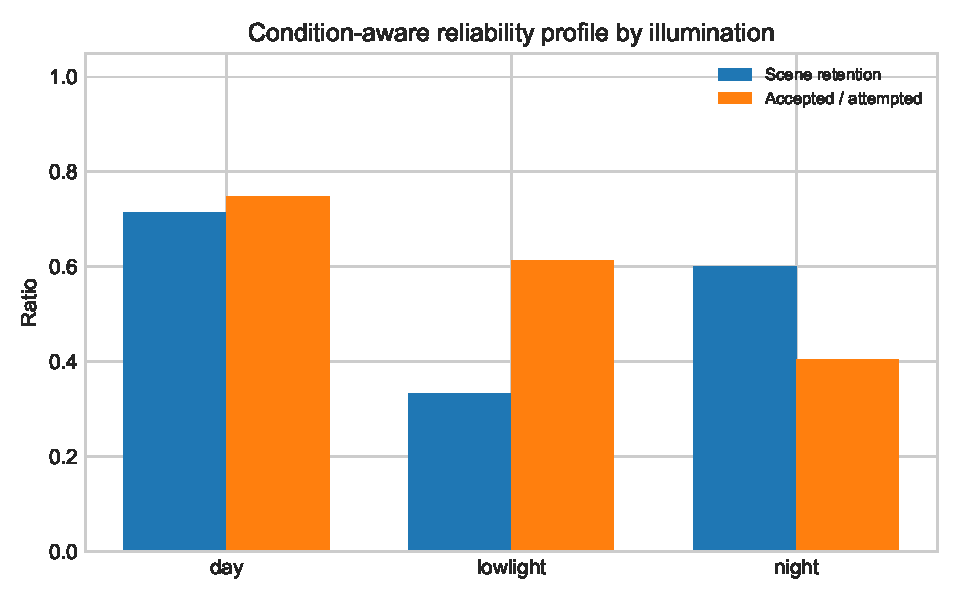
\includegraphics[width=0.78\textwidth]{figures/fig_condition_reliability_profile.pdf}
\caption{Condition-aware reliability profile by illumination. Scene retention and accepted-frame
support summarize complementary aspects of the retained alignment products.}
\label{fig:condition_reliability}
\end{figure}

\subsection{Reliability-Coverage Operating Profile}

The canonical QA gate defines retained alignment products, while the reliability score is used for
ranking, threshold sweep, and operating-profile visualization. The score-ranked top-$K$ subsets and
the canonical retained-scene set are related but not identical. Figure~\ref{fig:risk_coverage}
therefore marks the strict canonical 9/15 operating point explicitly while plotting the
score-ranked reliability--coverage curve.

\begin{figure}[t]
\centering
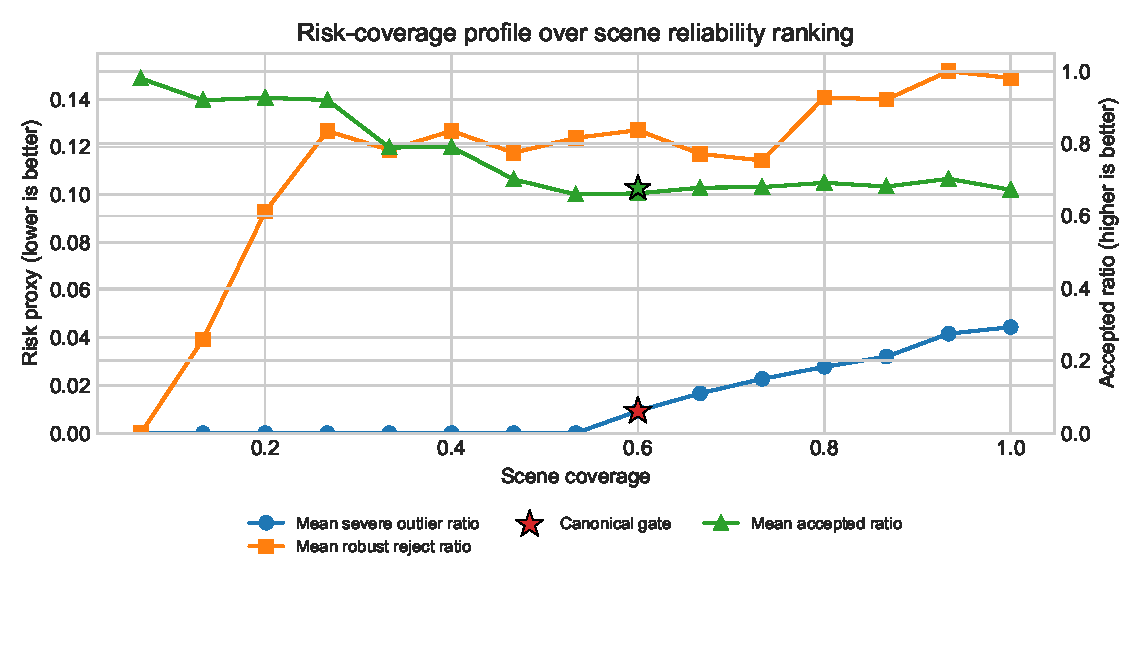
\includegraphics[width=0.82\textwidth]{figures/fig_risk_coverage_curve.pdf}
\caption{Risk-coverage operating profile on UAV-TAlign-12K. The curves are generated by ranking
scenes with the non-trained reliability score and progressively increasing retained coverage. The
star marks the strict canonical QA-gate operating point (9/15 retained scenes). The score-ranked
top-$K$ operating points visualize the reliability--coverage profile and do not replace the
canonical decision rule.}
\label{fig:risk_coverage}
\end{figure}

At the canonical point, UAV-TAlign retains 9 scenes, covers 60.0\% of scenes and 74.4\% of
evaluated pairs, and keeps the mean severe-outlier ratio at 0.009. The score-ranked curve exposes a
smooth operating profile from conservative high-confidence retention to broader inclusive
coverage. We keep the canonical gate fixed and use this curve to visualize the reliability--coverage
trade-off.

\subsection{Cumulative Ablation}

The accepted 8-scene supplement clarifies two complementary points. First, QA-aware verification
turns a permissive scene-pass pipeline into a retained-product decision rule. Second, the frame
selection policy matters primarily near the pass/fail boundary rather than through large changes
in overall accepted-frame support. On this subset, the candidate-only and consensus-only variants
both keep 8/8 scenes under the pre-verification criterion, whereas the deterministic-even
QA-aware variant contracts to 5/8 retained scenes.

\begin{table}[t]
\caption{Frozen cumulative ablation on the fixed 8-scene subset. The table emphasizes retained
product behavior under the accepted local supplement evidence.}
\label{tab:ablation_main}
\centering
\resizebox{\textwidth}{!}{
\begin{tabular}{lcccrrrr}
\toprule
Variant & Selection & Consensus & Verification & Retained/N $\uparrow$ & QA Pass/N $\uparrow$ & Acc. Mean $\uparrow$ & Acc. Range \\
\midrule
A1 candidate only & candidate-only & \xmark & \xmark & 8/8 & 5/8 & 13.6 & 8--34 \\
A2 + robust scene consensus & candidate-only & \cmark & \xmark & 8/8 & 5/8 & 13.6 & 8--34 \\
A3 + QA-aware verification & even & \cmark & \cmark & 5/8 & 5/8 & 26.0 & 7--49 \\
Random selection full (seed0) & random & \cmark & \cmark & 5/8 & 6/8 & 26.6 & 7--49 \\
\bottomrule
\end{tabular}}
\end{table}

The accepted random-selection supplement further shows a 5/8 to 7/8 spread across seeds on the
same fixed subset. The variation is concentrated in a small number of borderline scenes, while the
accepted-frame means remain comparatively stable across seeds. Deterministic-even selection
therefore serves as a reproducible default operating policy, and the multi-seed result is best
read as boundary sensitivity rather than full-pipeline instability.

\begin{figure}[t]
\centering
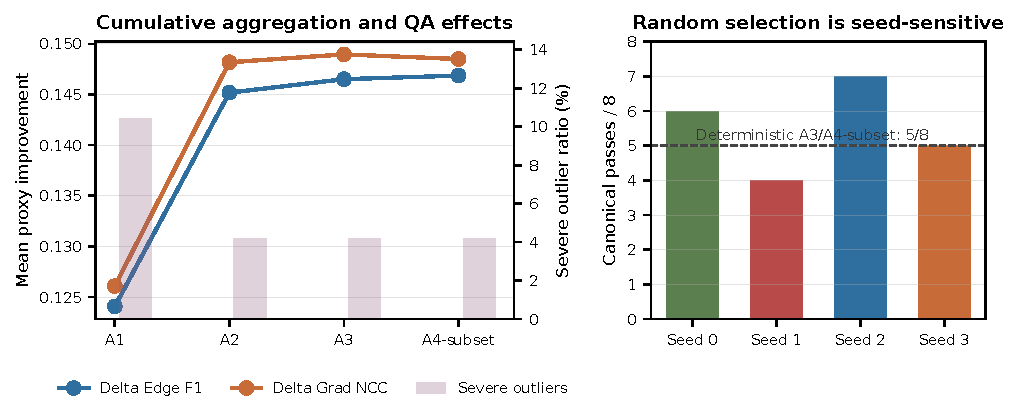
\includegraphics[width=\textwidth]{figures/fig_ablation_sensitivity.pdf}
\caption{Cumulative ablation and random-selection supplement. Robust scene consensus improves proxy
quality before the final gate, while the random-selection variant shows non-trivial seed
sensitivity on the same fixed 8-scene subset.}
\label{fig:ablation_sensitivity}
\end{figure}
